\chapter*{Vorwort}
Zu Beginn dieses Kurses wollen wir uns eine bedeutende und tiefgreifende Wahrheit erkennen und in unserem Innersten verankern:

\begin{center}
\begin{Huge}
	\emph{Computer sind strunzdumm.}
\end{Huge}
\end{center}

Im Wesentlichen ist das auch ganz gut so. Wäre dem nicht so, könnten wir Ihnen nicht die Aufgaben überlassen, die uns zu lästig sind. Wie jeder weiß, der an einen weniger bemittelten Zeitgenossen Teile seiner Arbeit deligieren wollte, müssen die Anweisungen dann aber auf den Punkt exakt formuliert sein. Für Computer gilt das nur umso mehr. In den Übungsstunden der Programmierpraktika höre ich von KursteilnehmerInnen immer wieder so etwas wie \emph{Ich dachte, der Computer würde verstehen dass...}, worauf ich gerne antworte: \emph{Du dachtest -- er nicht.}

Die Programmiersprache \emph{Python} wurde entwickelt, um gerade diese Schwierigkeit am Programmieren \emph{etwas} abzumildern. Der Interpreter (also das Programm, das den Programmcode in Elektronik-Anweisungen übersetzt) erkennt viele implizite Angaben, die in anderen Sprachen mühevoll ergänzt werden müssten. Dies macht die Sprache gerade für AnwenderInnen attraktiv, die sich nicht primär als Programmierer\-Innen verstehen. Anstatt sich mit Speicherstrukturen und Datenflüssen zu beschäftigen, kann bei der Entwicklung in Python das Hauptaugenmerk auf dem übergeordneten Problem bleiben. Viele regelmäßig wiederkehrede Aufgaben sind in Python bereits gelöst und können als Standardbaublöcke in eigene Codes eingebaut werden. Dieses Sprachdesign veranlasste Randall Munroe\footnote{Autor des legendären Webcomics \emph{xkcd} und der Bücher \emph{what if} und \emph{how to}. Falls Sie diese noch nicht kennen, füllen Sie diese Wissenslücke schnell auf -- es lohnt sich!} zur Veröffentlichung dieses Strips:

\begin{center}
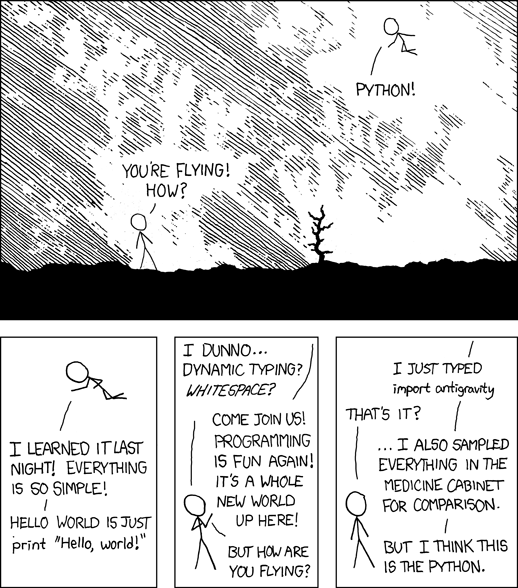
\includegraphics[width=.4\linewidth]{./gfx/xkcd-python}
\captionof{figure}
	[Antigravity in Python]
	{Antigravity in Python. Quelle: \url{https://xkcd.com/353/}}
\end{center}

Diese Euphorie soll nicht darüber hinweg täuschen, dass wir uns der schwierigen Aufgabe stellen, einem Computer unseren Willen abzuverlangen. Aber ähnlich wie Randall Munroe und ich werden Sie beim Erlernen dieser Fähigkeit mit Python schnell Erfolgserlebnisse haben und sicher Spaß daran finden.

Dieses Script soll Sie in der Vorlesung \emph{\myTitle} im \currentPeriod begleiten. Alle wichtigen Kursinhalte werden hier behandelt und anhand von Beispielen verdeutlicht. Es versteht sich von selbst, dass ein optimaler Lernerfolg nur bei Besuch der Vorlesung gegeben ist. Vorkenntnisse in anderen Programmiersprachen sind zur Arbeit mit diesem Script nicht notwendig.

Hier wird von einer Linux-Arbeits\-umgebung ausgegangen und minimale Grundkenntnisse dieser Arbeits\-umgebung vorausgesetzt (Starten einer Kommandozeilen-Umgebung, Wechsel des Arbeitsverzeichnisses, Aufrufen von Programmen aus der Kommandozeile, Übergabe von Parametern an Programme). Die DozentInnen des Kurses können bei Bedarf erklären, wie die Arbeitsumgebung bedient wird.

Dieses Dokument ist keine vollständige Referenz der Sprache Python. Hier sollen nur die Grundlagen des Programmierens in Python vermittelt werden. Als Standard-Nachschlagewerk empfehle ich die offizielle Dokumentation\url{https://docs.python.org/3/} (englisch). Zum einen finden Sie dort ausführliche und vollständige Erklärungen zu allen Themen, die Ihnen bei der Arbeit mit \emph{Python} begegnen können. Zum anderen haben Sie sicherlich Freude an den vielen Anspielungen auf die Sketche der Britischen Anarcho-Komiker \emph{Monty Python}\footnote{\emph{Das Leben des Brian} und \emph{Die Ritter der Kokosnuß}\footnotemark \;
sollten sie unbedingt sehen!}, nach denen die Sprache benannt ist.
\footnotetext{Ja, die Filme sind so alt, dass man damals \emph{Kokosnuß} noch mit scharfem ß schrieb.} 

Dieses Script wurde nach bestem Wissen und Gewissen zusammengestellt; Code-Beispiele wurden auf wenigstens einer Maschine getestet. Dennoch können menschliche Fehler nicht ausgeschlossen werden. Wem Unstimmigkeiten auffallen oder wer Vorschläge und Anregungen zu diesem Text einbringen will, möge mir dies sehr gerne mitteilen. Ich bin erreichbar unter meiner Email-Adresse:\\ \url{stefan.hartinger@stud.uni-regensburg.de}.
\begin{flushright}
\myName, \myVersionTime
\end{flushright}